\section{Introduction}
Analog circuit simulation (Figure \ref{fig:simulator-flowchart}) \cite{nagel1971computer,mccalla1971bias,Nagel:M382} has become one of the most important tools in the analog circuit EDA toolchain to assist verification and design. This is due to long-term research accumulation in algebraic differential equation theory \cite{estevez2000structural,kunkel2006differential,gunther2005modelling}, device modeling \cite{chauhan2012bsim,ezaki2008physics,gildenblat2006psp}, equations system construction \cite{hachtel1971sparse,ho1975modified,fijnvandraat2002time}, nonlinear equations solvers \cite{nastov2007fundamentals,najm2010circuit}, hardware description languages (HDLs) \cite{verilog2014verilog,ieee2006ieee-1364-2005,lemaitre2002adms,christen1999vhdl,pecheux2005vhdl}, and more.
\begin{figure}[htpb]
	\centering
	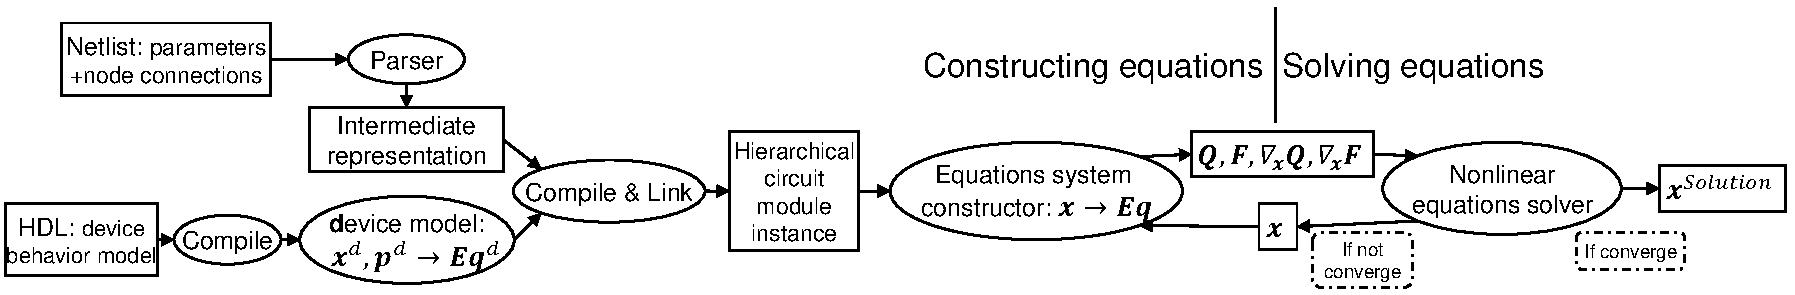
\includegraphics[width=1.0\textwidth]{fig/simulator-flowchart.pdf}
	\caption{Simulator flowchart}
	\label{fig:simulator-flowchart}
\end{figure}
However, we still see inconveniences with popular HDLs and simulators in reusing coarse-grained circuit module behavior models, introducing multi-physical effects, and applying gradient optimization methods to automatic design.
\begin{itemize}[partopsep=0pt,topsep=0pt,itemsep=0pt,parsep=0pt]
	\item
	For device and circuit modeling, HDL technology is often used to create a device behavior model, which is then compiled \cite{lemaitre2002adms} into a program that the simulator can invoke. In particular, multi-port circuit behavior modeling often goes through two steps: function fitting and HDL implementation, for example, neural network fitting \cite{meijer2001neural,zhang2017artificial}+HDL or Volterra polynomial \cite{zhang2014large}+SPICE netlists \cite{zhang2019new,roymohapatra2019novel}.
	\item
	To achieve an optimal combination of circuit parameters in the automation of analog circuit design \cite{razavi2002design,silveira1996g,jespers2009gm}, it is necessary to first optimize the device size. Prior to 2010, researchers developed solutions based on gradient optimization using parameter sensitivity analysis \cite{zhan2004optimization,agrawal2006circuit}. To tune design variables, modern process and software technologies require that software uses callbacks to modify model parameters. However, such an approach hinders users from obtaining gradient information of the variables. This has pushed recent research to shift its focus toward black-box methods, such as local sampling for gradient reconstruction \cite{huang2013efficient,nieuwoudt2005multi,peng2016efficient}, surrogate models \cite{girardi2011analog,lyu2018batch,wang2014enabling,lyu2017efficient}, and reinforcement learning \cite{tang2018parametric}.
\end{itemize}
Many works attempt to address the above inconveniences from both the model compilation and the gradient acquisition perspectives. For example, \citet{mahmutoglu2018new} developed the Verilog-AMS compiler that can run using Matlab/Octave, \citet{kuthe2020verilogae} can obtain more information about the equations and internal derivatives when the Verilog-AMS circuit module is compiled, and \citet{hu2020adjoint} provides an efficient implementation of adjoint equations for transient simulation. However, none of these works explore functional support possibilities from the perspective of systems equations construction.

Indeed, one significant cause of these inconveniences is that the analog HDLs contain many complex and even bloated features, which are necessary for these HDLs to simultaneously support the representation of structural and behavioral information. Such features include the automatic differentiation required for analog simulation, and polynomial interpolation that may be used in modeling \cite[Sections 4.5.6, 9.21]{verilog2014verilog}. The intertwining of structural and behavioral information has isolated analog HDLs from the open ecosystems of other programming languages and tools, and also created high barriers for developing analog EDA tools. Furthermore, only static circuit parameters independent of signal values can be passed between nested circuit modules and simulation runtime variables are allowed only within modules (\cite[Sections 3.4, 6]{verilog2014verilog},\cite[Section 4.10]{ieee2006ieee-1364-2005}) --- this is not conducive to reuse and development of coarse-grained circuit models.

Thriving technologies such as deep learning \cite{goodfellow2016deep} and automatic differential programming \cite{baydin2018automatic} have contributed to a number of research fields in scientific computing, including data-driven multi-scale modeling and inverse problems \cite{zhang2018deep,long2018pde,long2019pde}. Inspired by such works, this paper proposes a computational graph implementation of an equations system constructor that works in hierarchical circuit simulation \cite{fijnvandraat2002time,ter1999numerical,mukherjee1999hierarchical,tcherniaev2003transistor}, along with the corresponding JSON netlist and compilation method (Figure \ref{fig:flowchart}). The internal and external variables, design variables, model input parameters, and corresponding gradients of circuit modules are processed in a unified manner.
This work takes circuit modules as the basic units of a computational graph and supports decoupled representation of circuit models using "equivalent circuit decomposition using JSON netlist+submodel for computing dynamic parameters". The advantages of this approach are twofold: (1) JSON format is easy to parse, and its basic data types "dictionary+list" are sufficient to represent circuit structure information. And (2), a submodel can be implemented with the help of the automatic differentiation capability of Julia\cite{Bezanson_Julia_A_fresh_2017}. Based on these two advantages, the proposed method in this paper simplifies circuit modeling and enhances the gradient acquisition capability of simulation tools.
\begin{figure}[htpb]
	\centering
	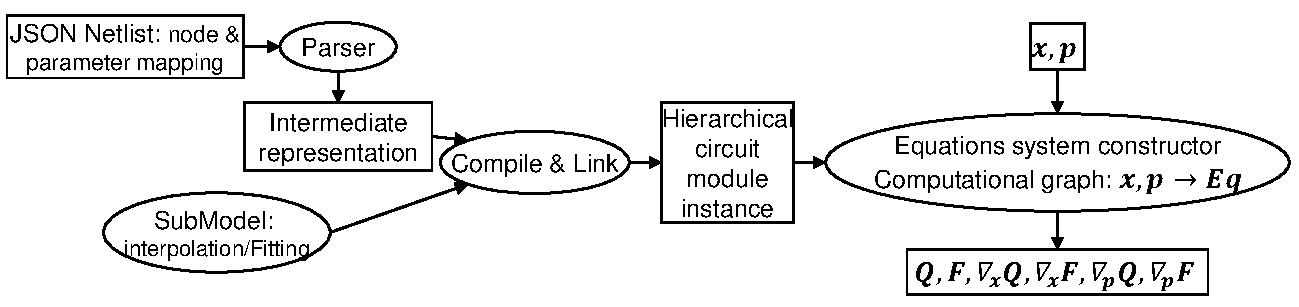
\includegraphics[width=0.7\textwidth]{fig/flowchart.pdf}
	\caption{Flowchart: create computational graph from a JSON netlist}
	\label{fig:flowchart}
\end{figure}

Section \ref{sec:Joanna} describes the processing of structural information related to circuit modules in a computational graph. Similar to defining, compiling, representing, and executing functions in a programming language \cite{aho2007compilers,muchnick1997advanced,appel2004modern}, the process involves the following steps:
module definition (netlist), parsing and compilation, data structures of module instances, and graph executor (Figure \ref{fig:equations-system-constructor}). Additionally, Section \ref{subsec:EvalCompositeSubCkt} introduces how to define and use SubModel for computing intrinsic dynamic parameters to provide behavioral information of each circuit module. Section \ref{sec:applications} presents two application examples, one for device modeling and the other for a joint solution of DC/AC analysis and device sizing under different process, voltage, and temperature (PVT) combinations.


